\pagenumbering{arabic}
\section{DES加解密算法}
\begin{figure}[thbp!]
	\centering
	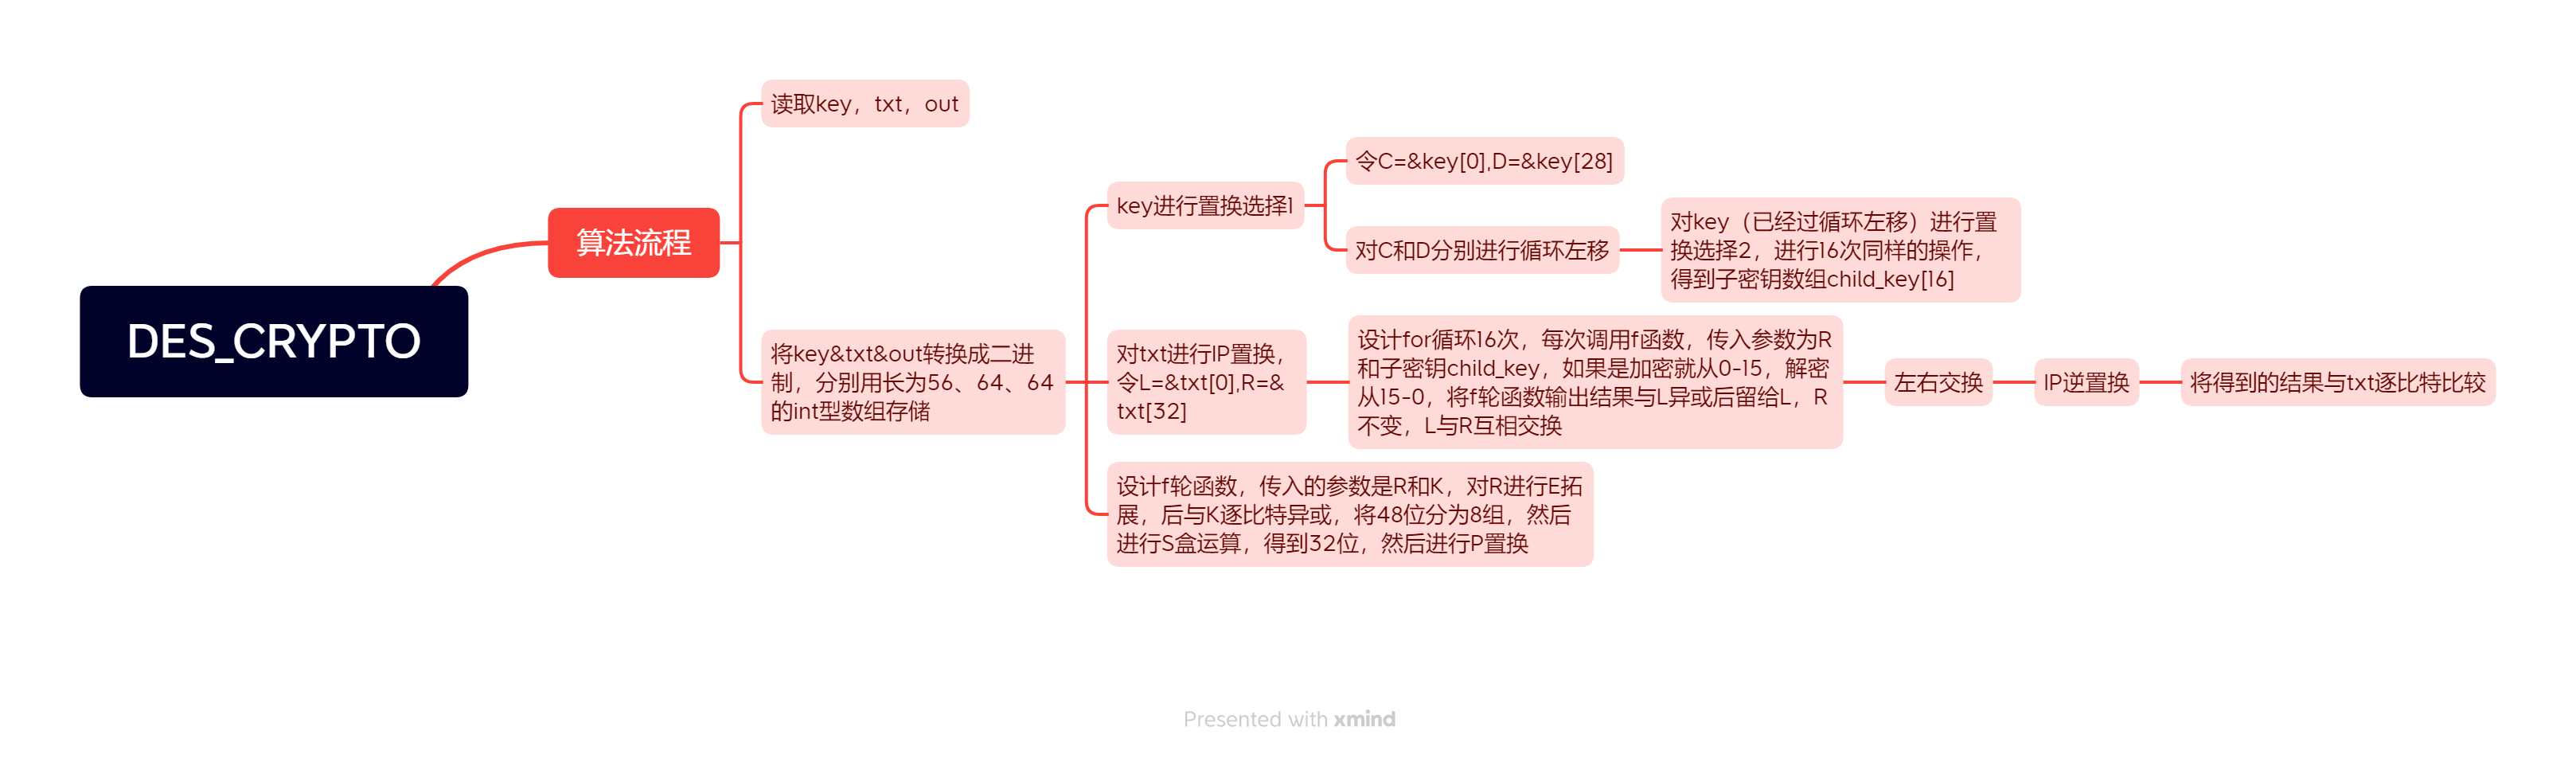
\includegraphics[height=6 CM,width=18cm]{figure/001}
	\caption{DES算法流程图}
	\label{fig:DES算法流程图}
\end{figure}
\begin{figure}[thbp!]
	\centering
	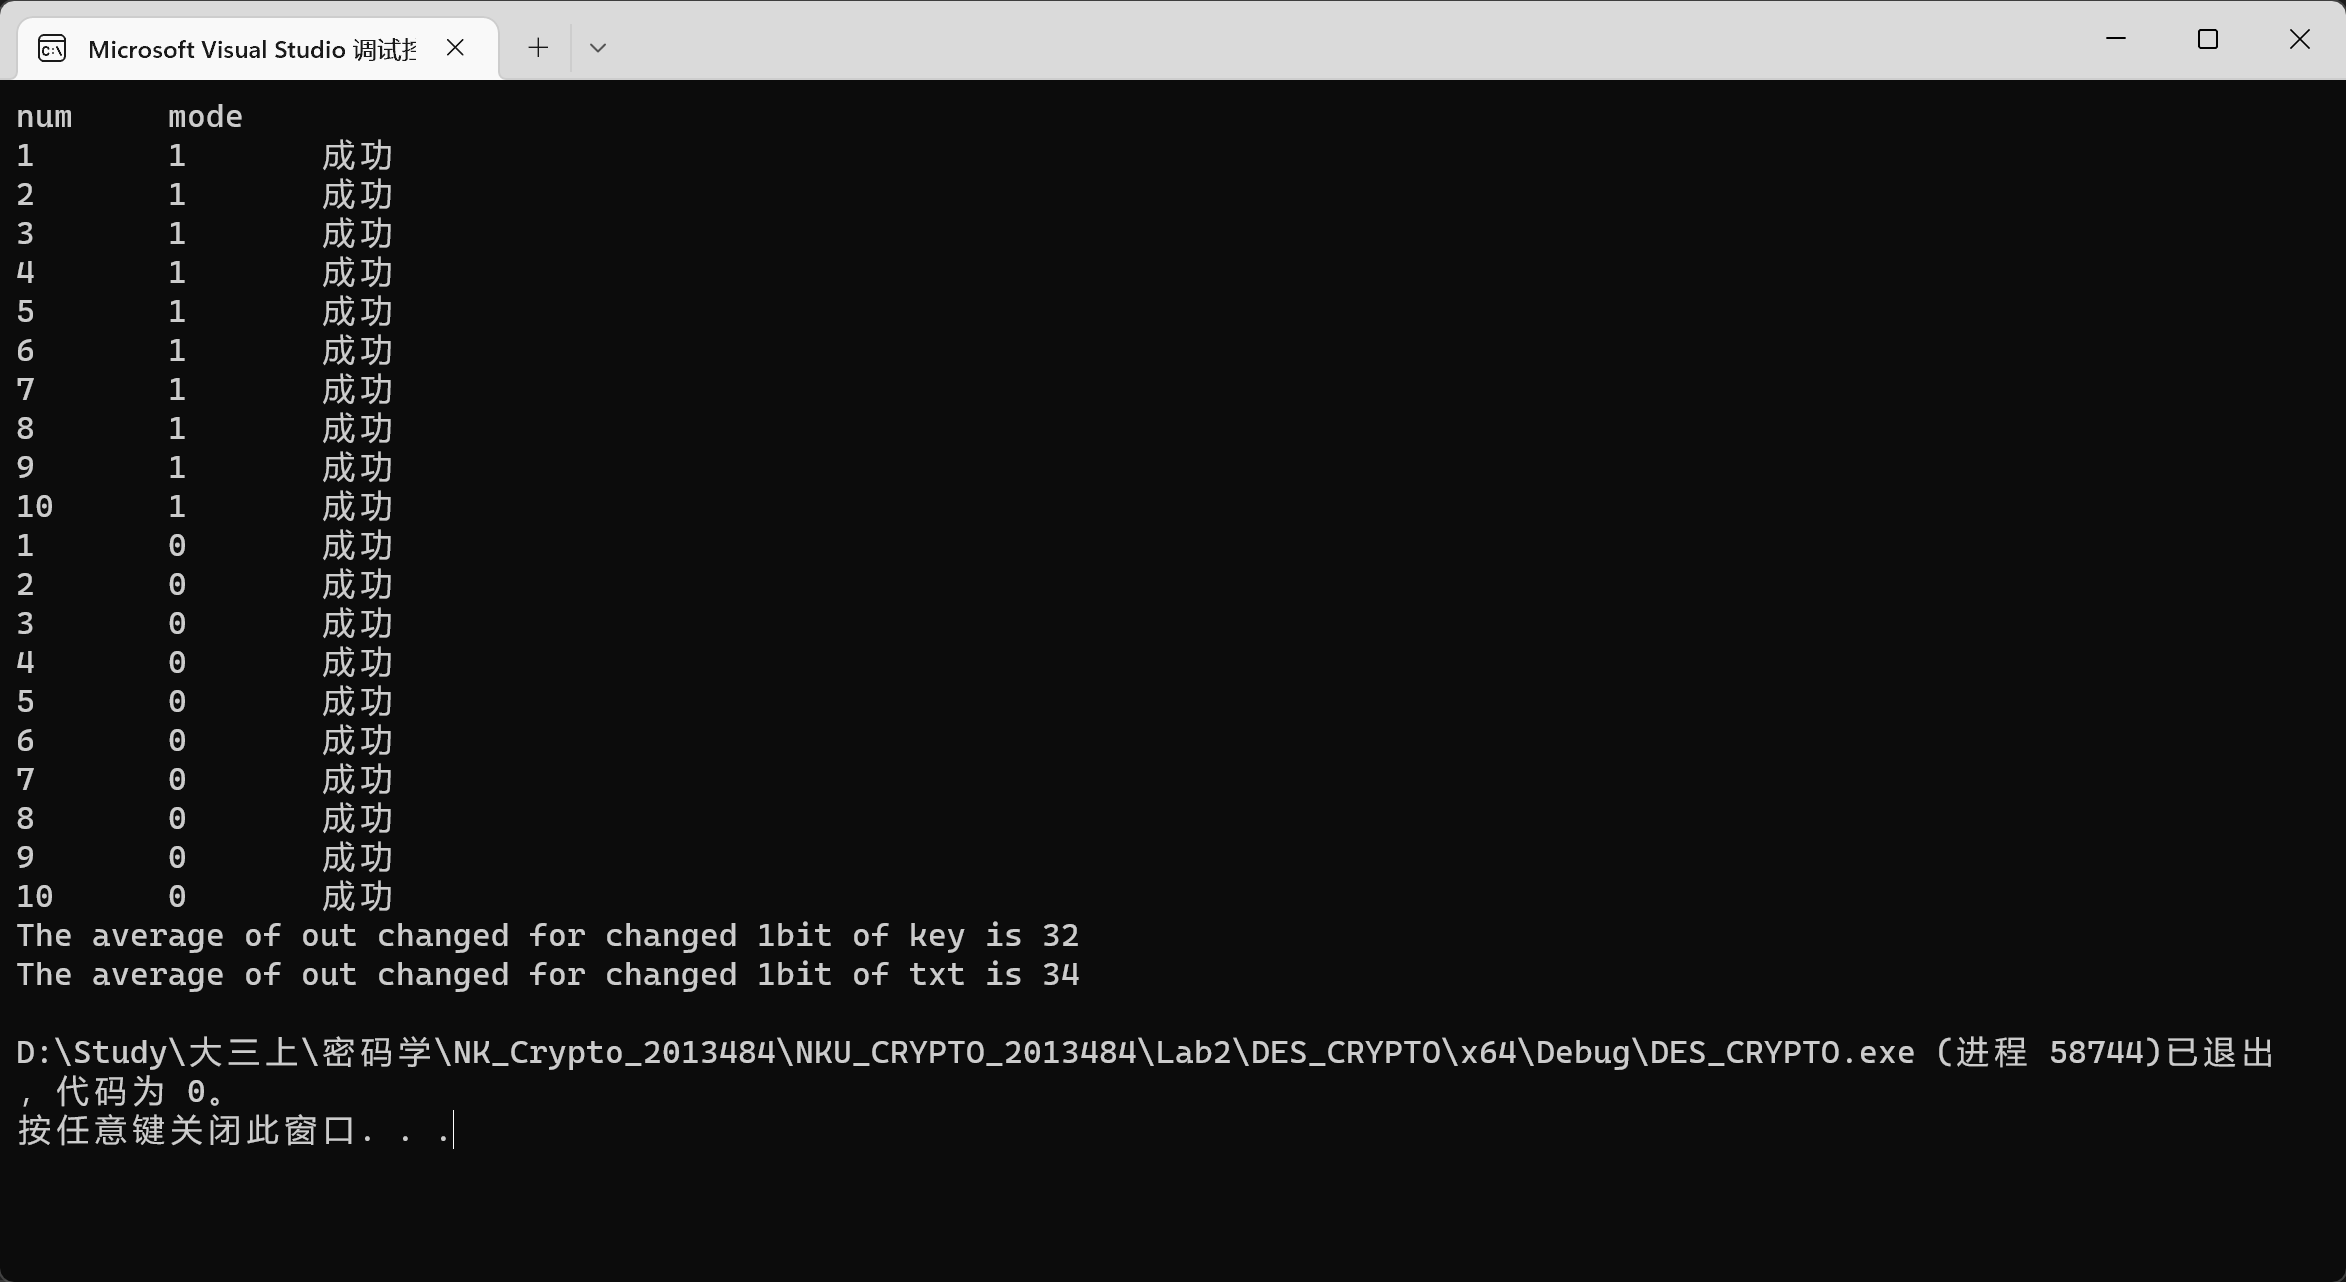
\includegraphics[height=10 CM]{figure/002}
	\caption{输出结果演示}
	\label{fig:输出结果演示}
\end{figure}

20组样例全部正确,改变key1位,8次得到的平均值是32,改变txt1位,8次计算得到的平均值是34\\

接下来概括性写一下中间生成结果(以第一组数据为例)\\
\begin{figure}[thbp!]
	\centering
	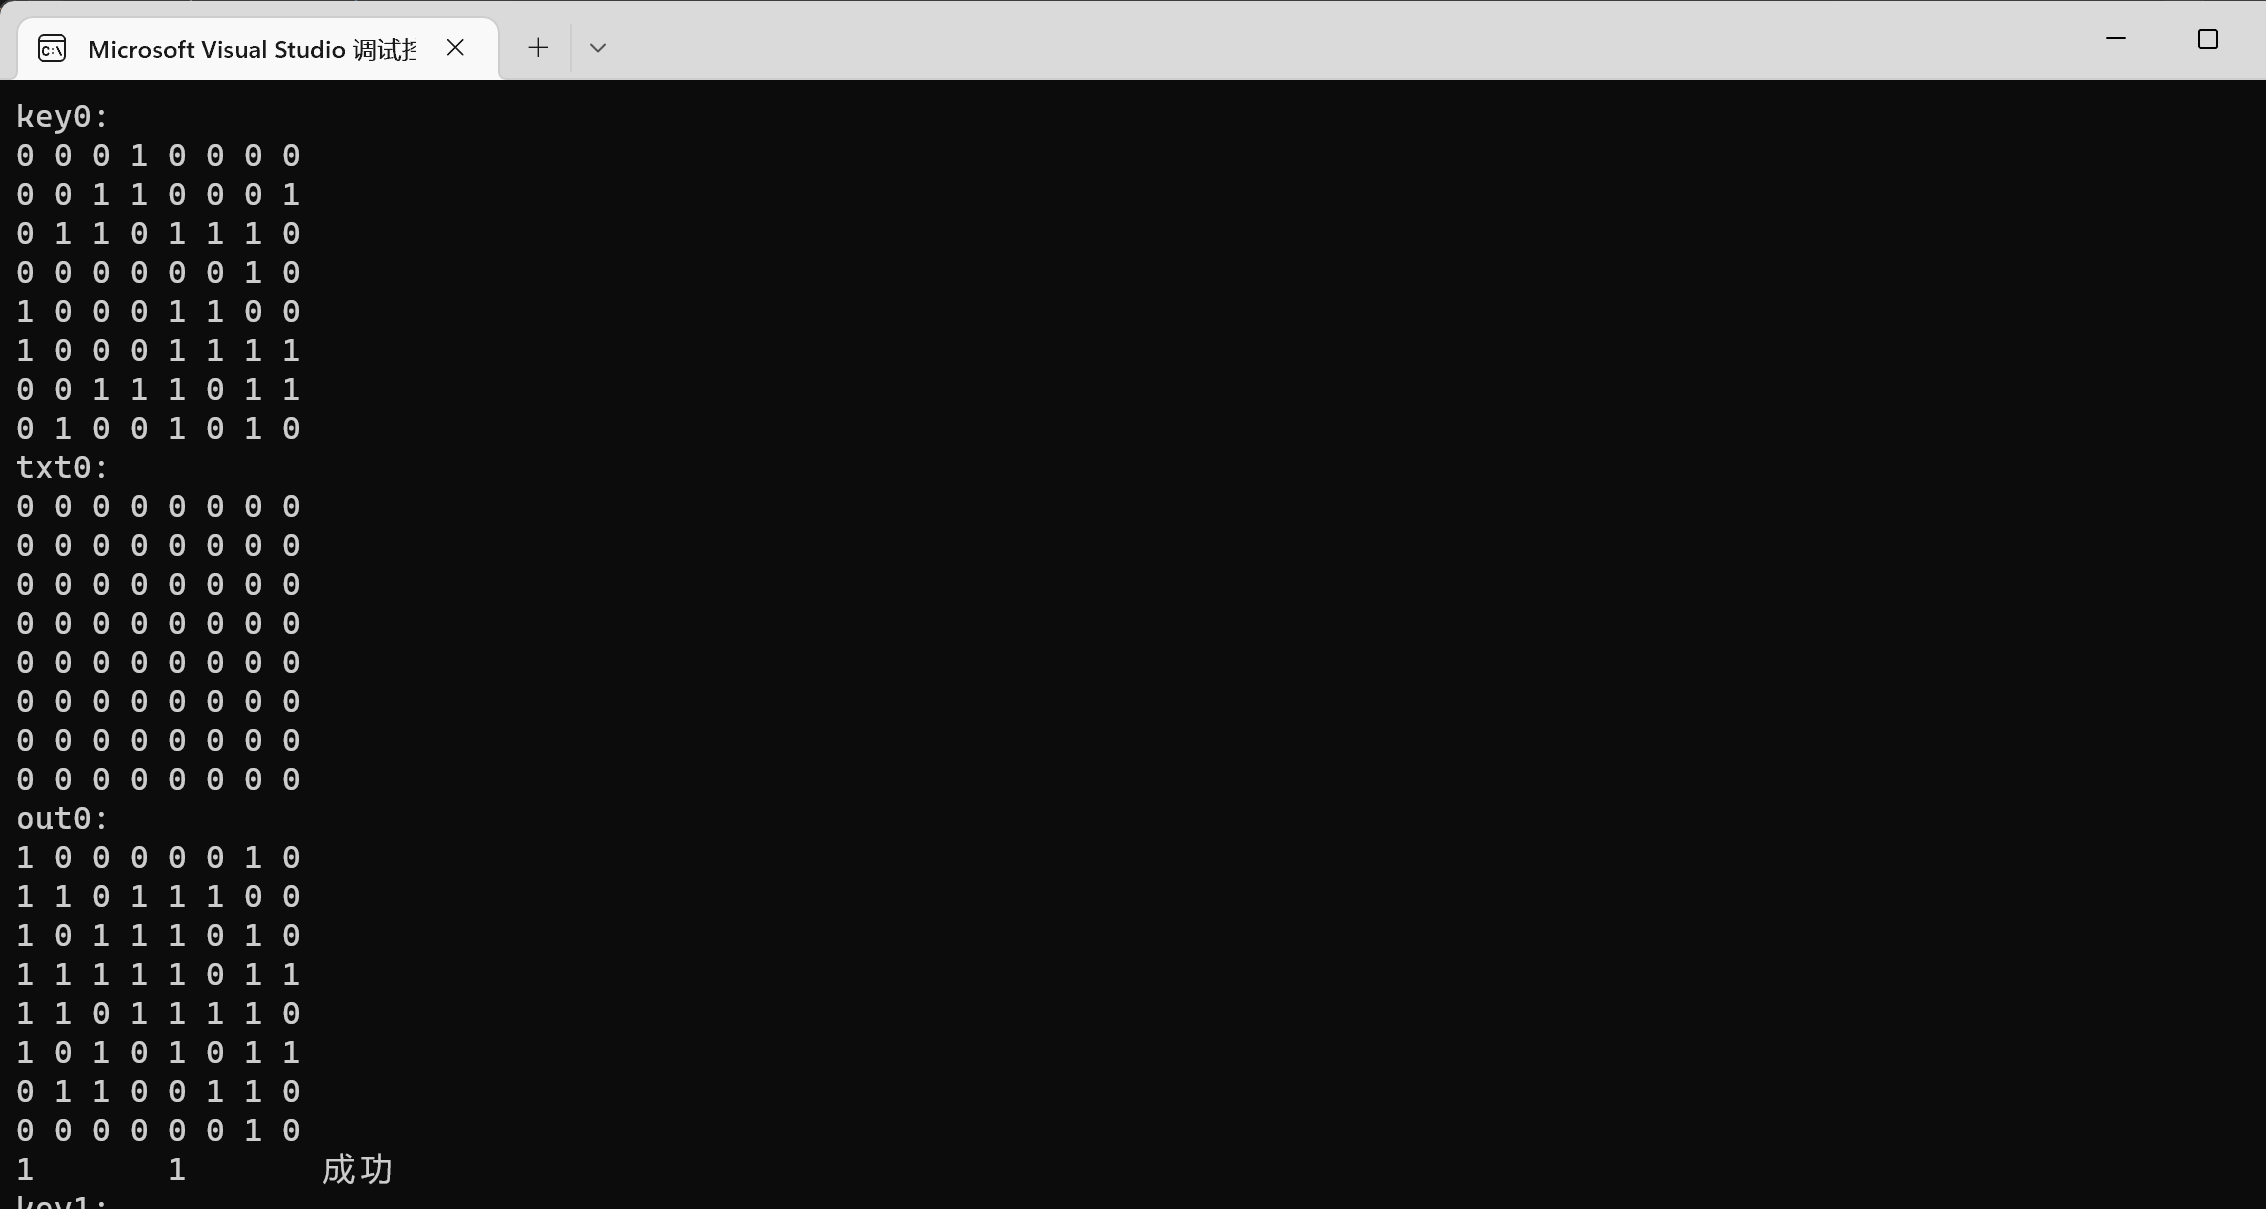
\includegraphics[height=10 CM]{figure/003}
	\caption{读入的第一组数据}
	\label{fig:读入的第一组数据}
\end{figure}
\begin{figure}[thbp!]
	\centering
	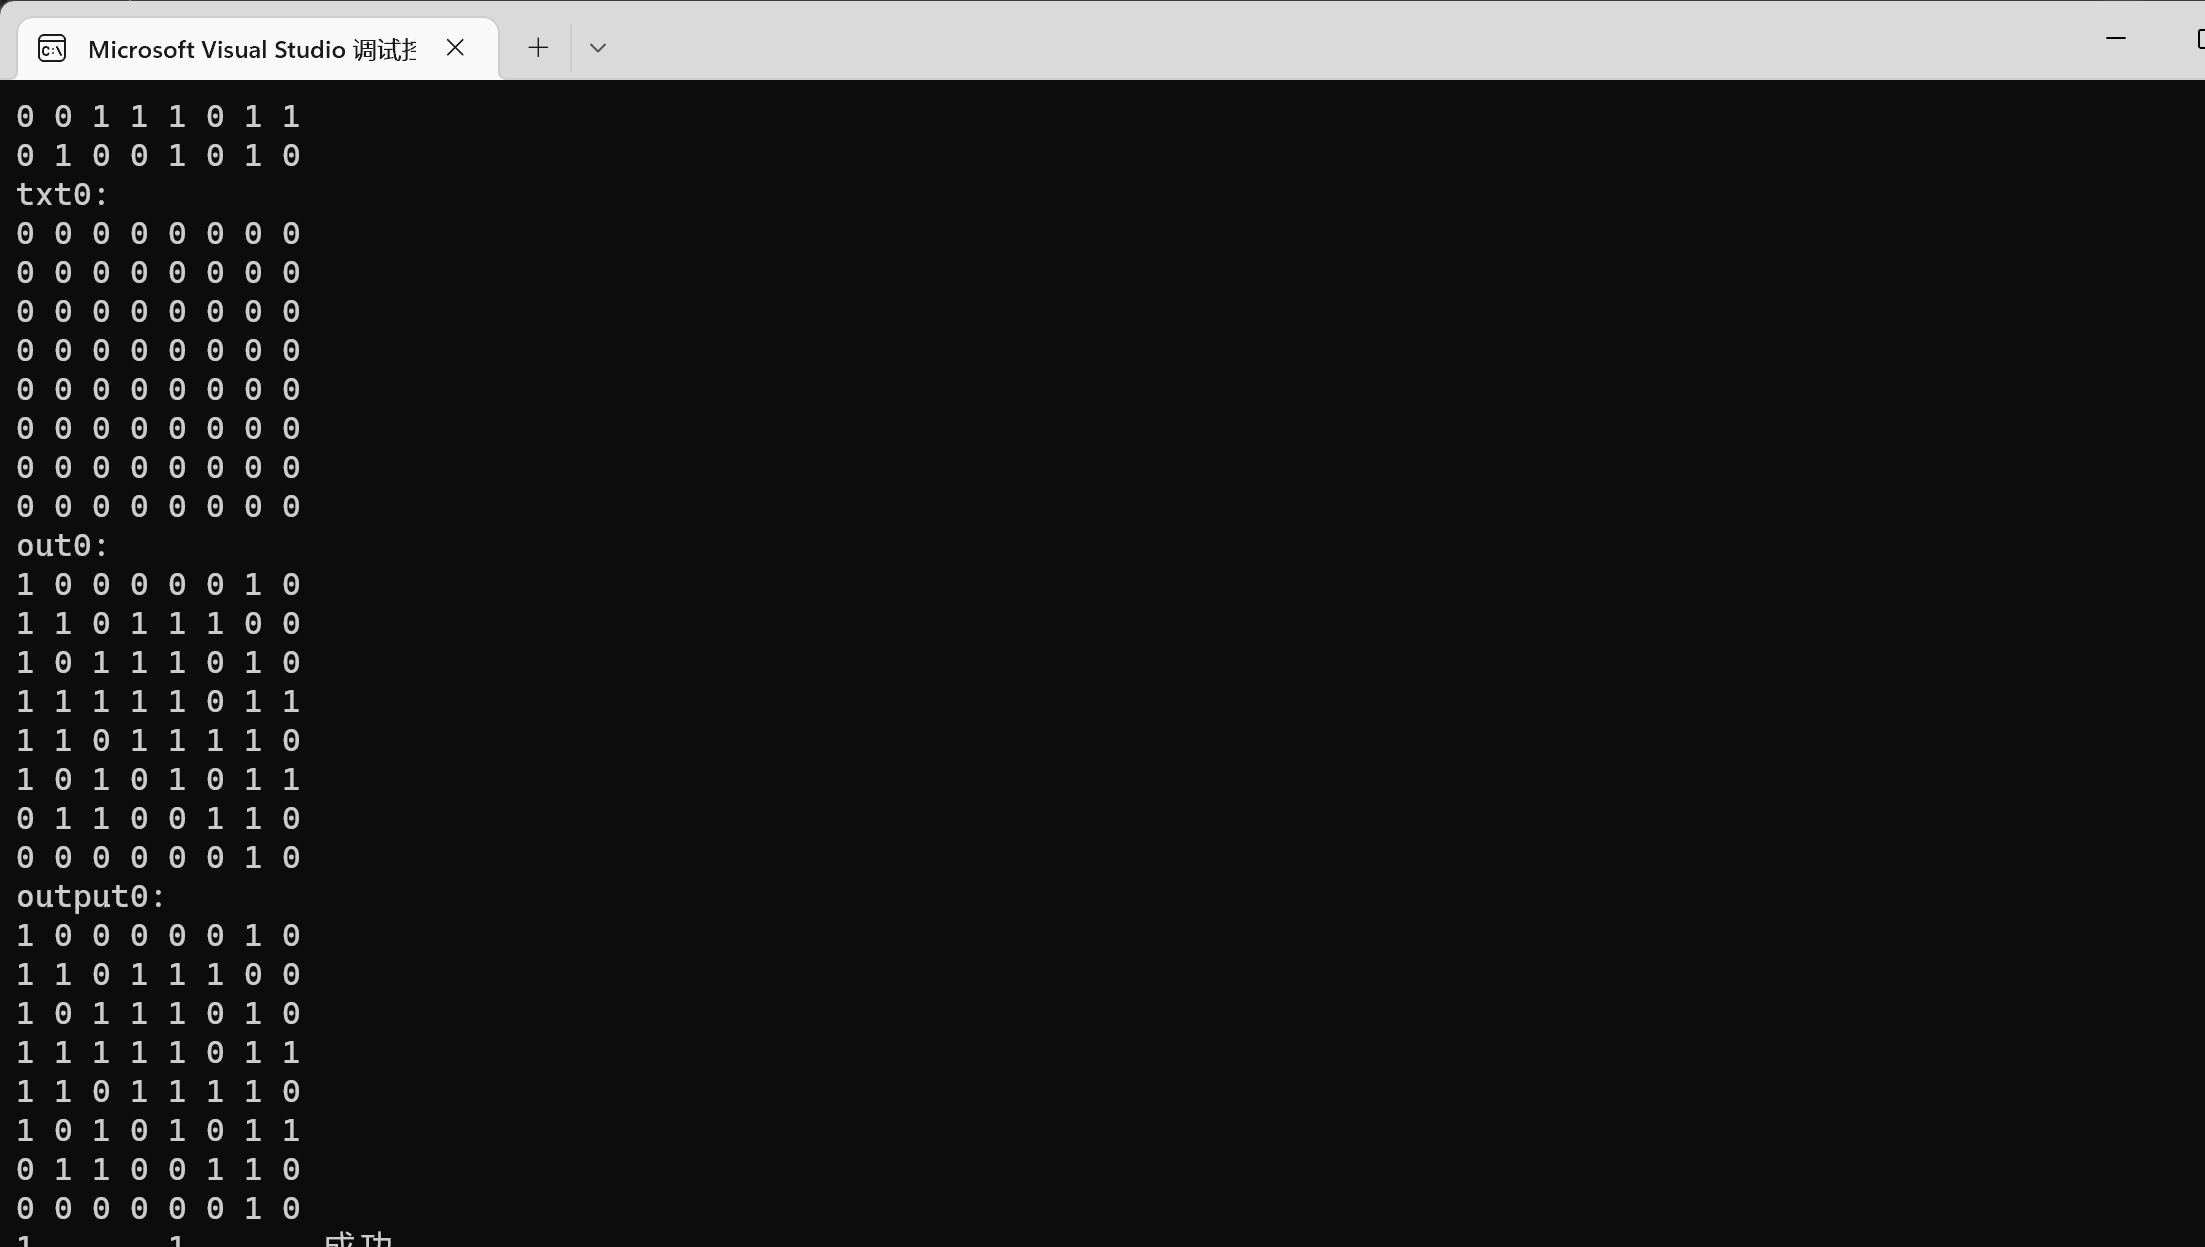
\includegraphics[height=10 CM]{figure/004}
	\caption{第一组计算结果与标准结果一致}
	\label{fig:第一组计算结果与标准结果一致}
\end{figure}
\begin{figure}[thbp!]
	\centering
	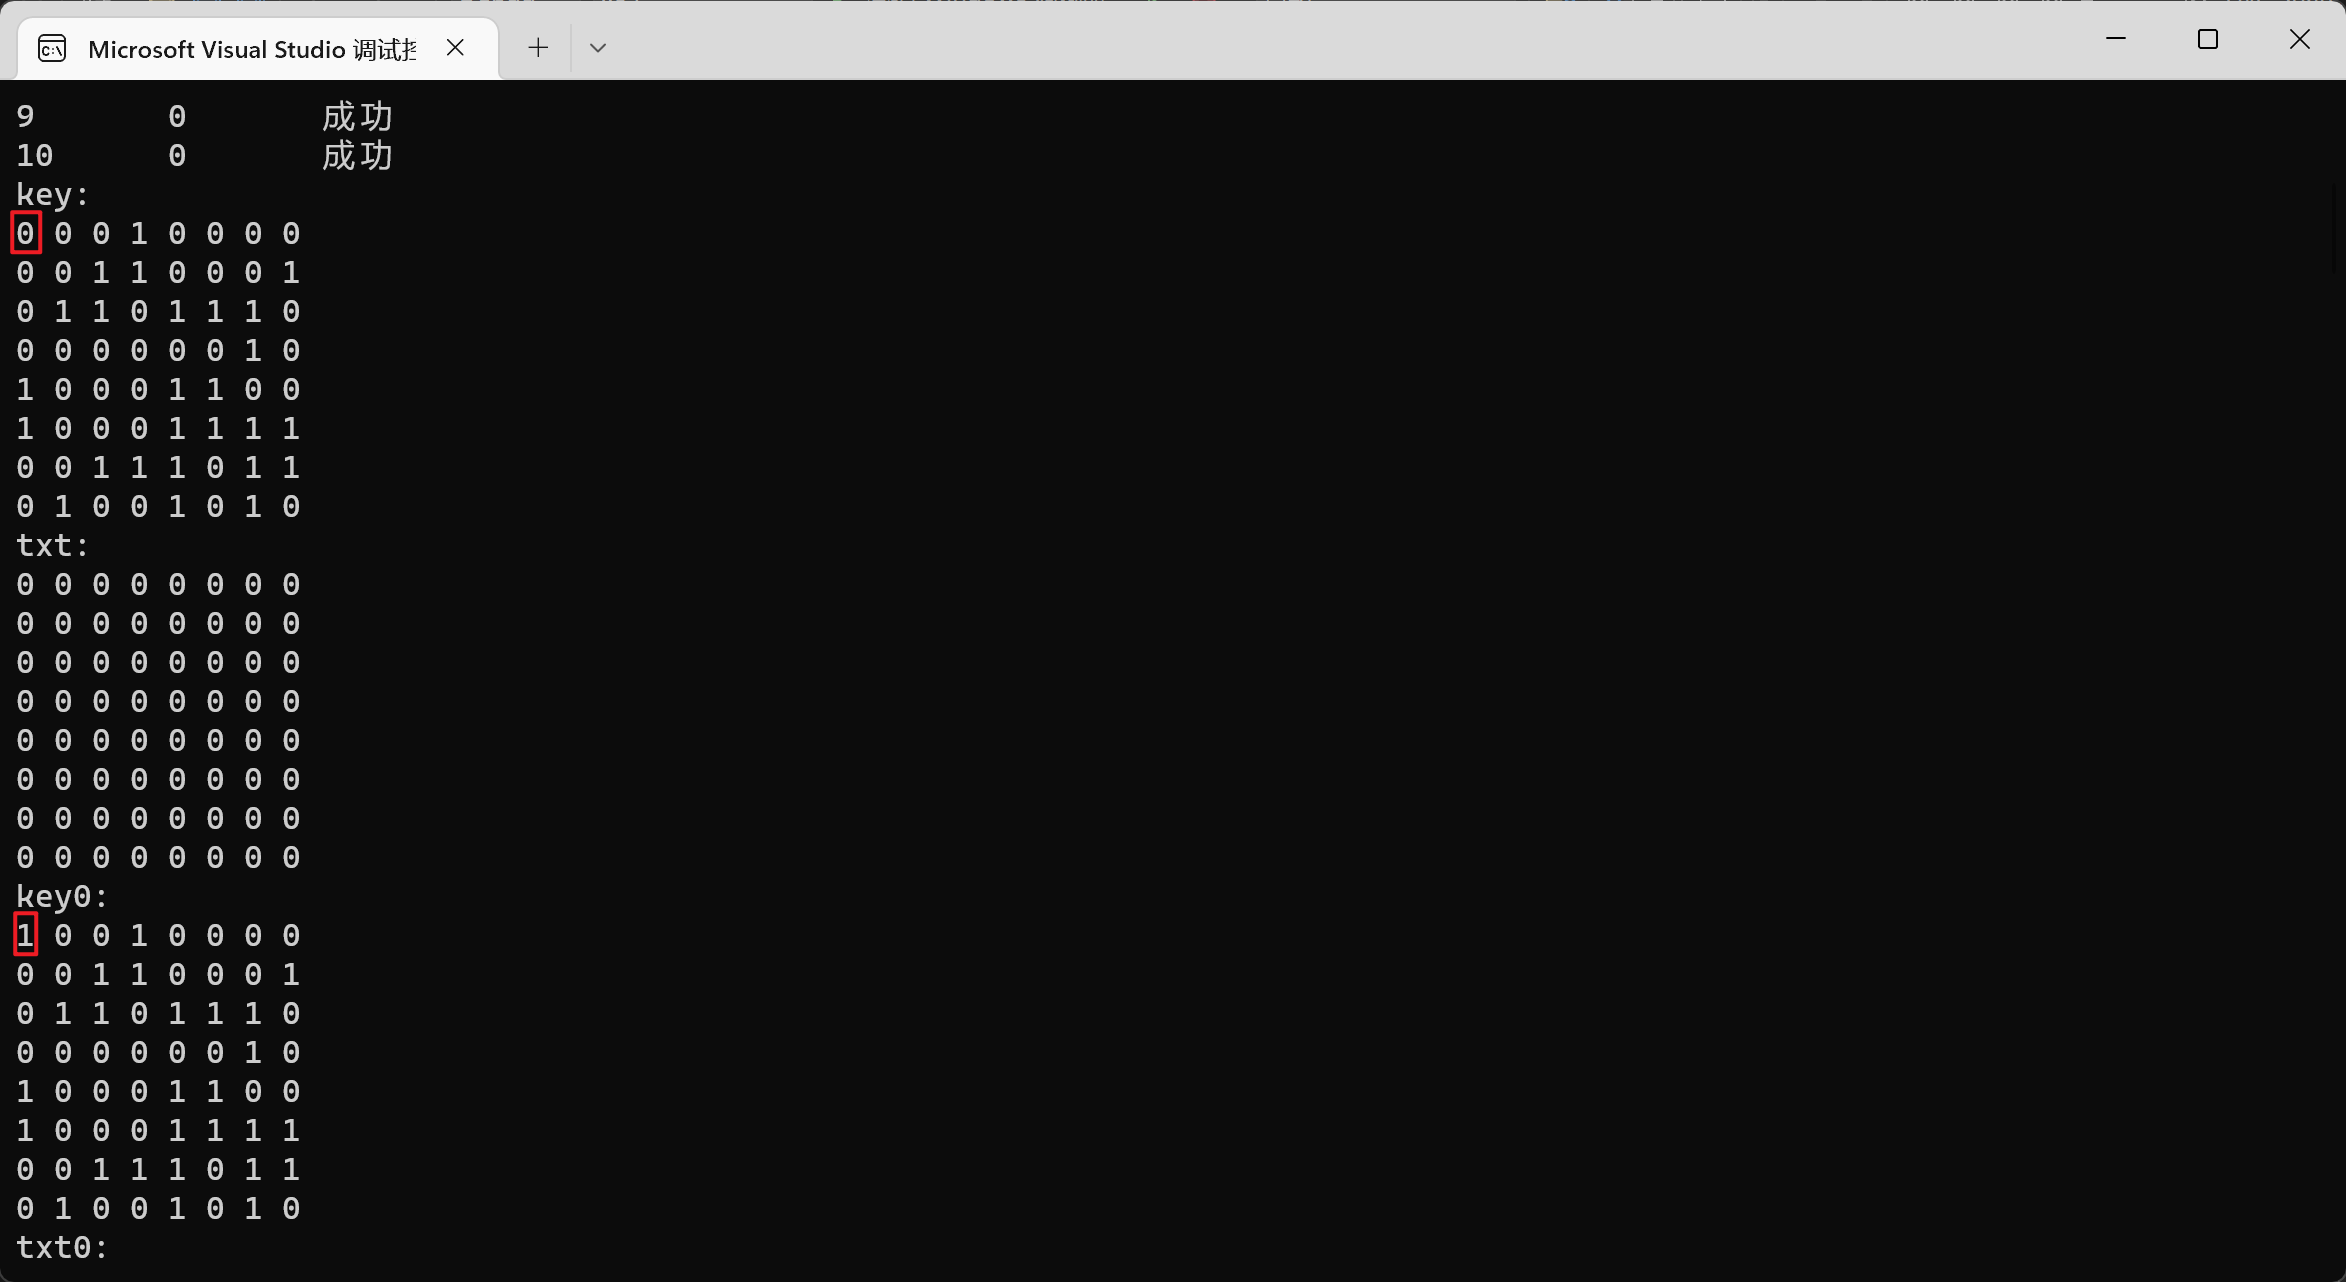
\includegraphics[height=10 CM]{figure/005}
	\caption{计算雪崩效应,改变key的一位,txt不变}
	\label{fig:计算雪崩效应,改变key的一位,txt不变}
\end{figure}
\begin{figure}[thbp!]
	\centering
	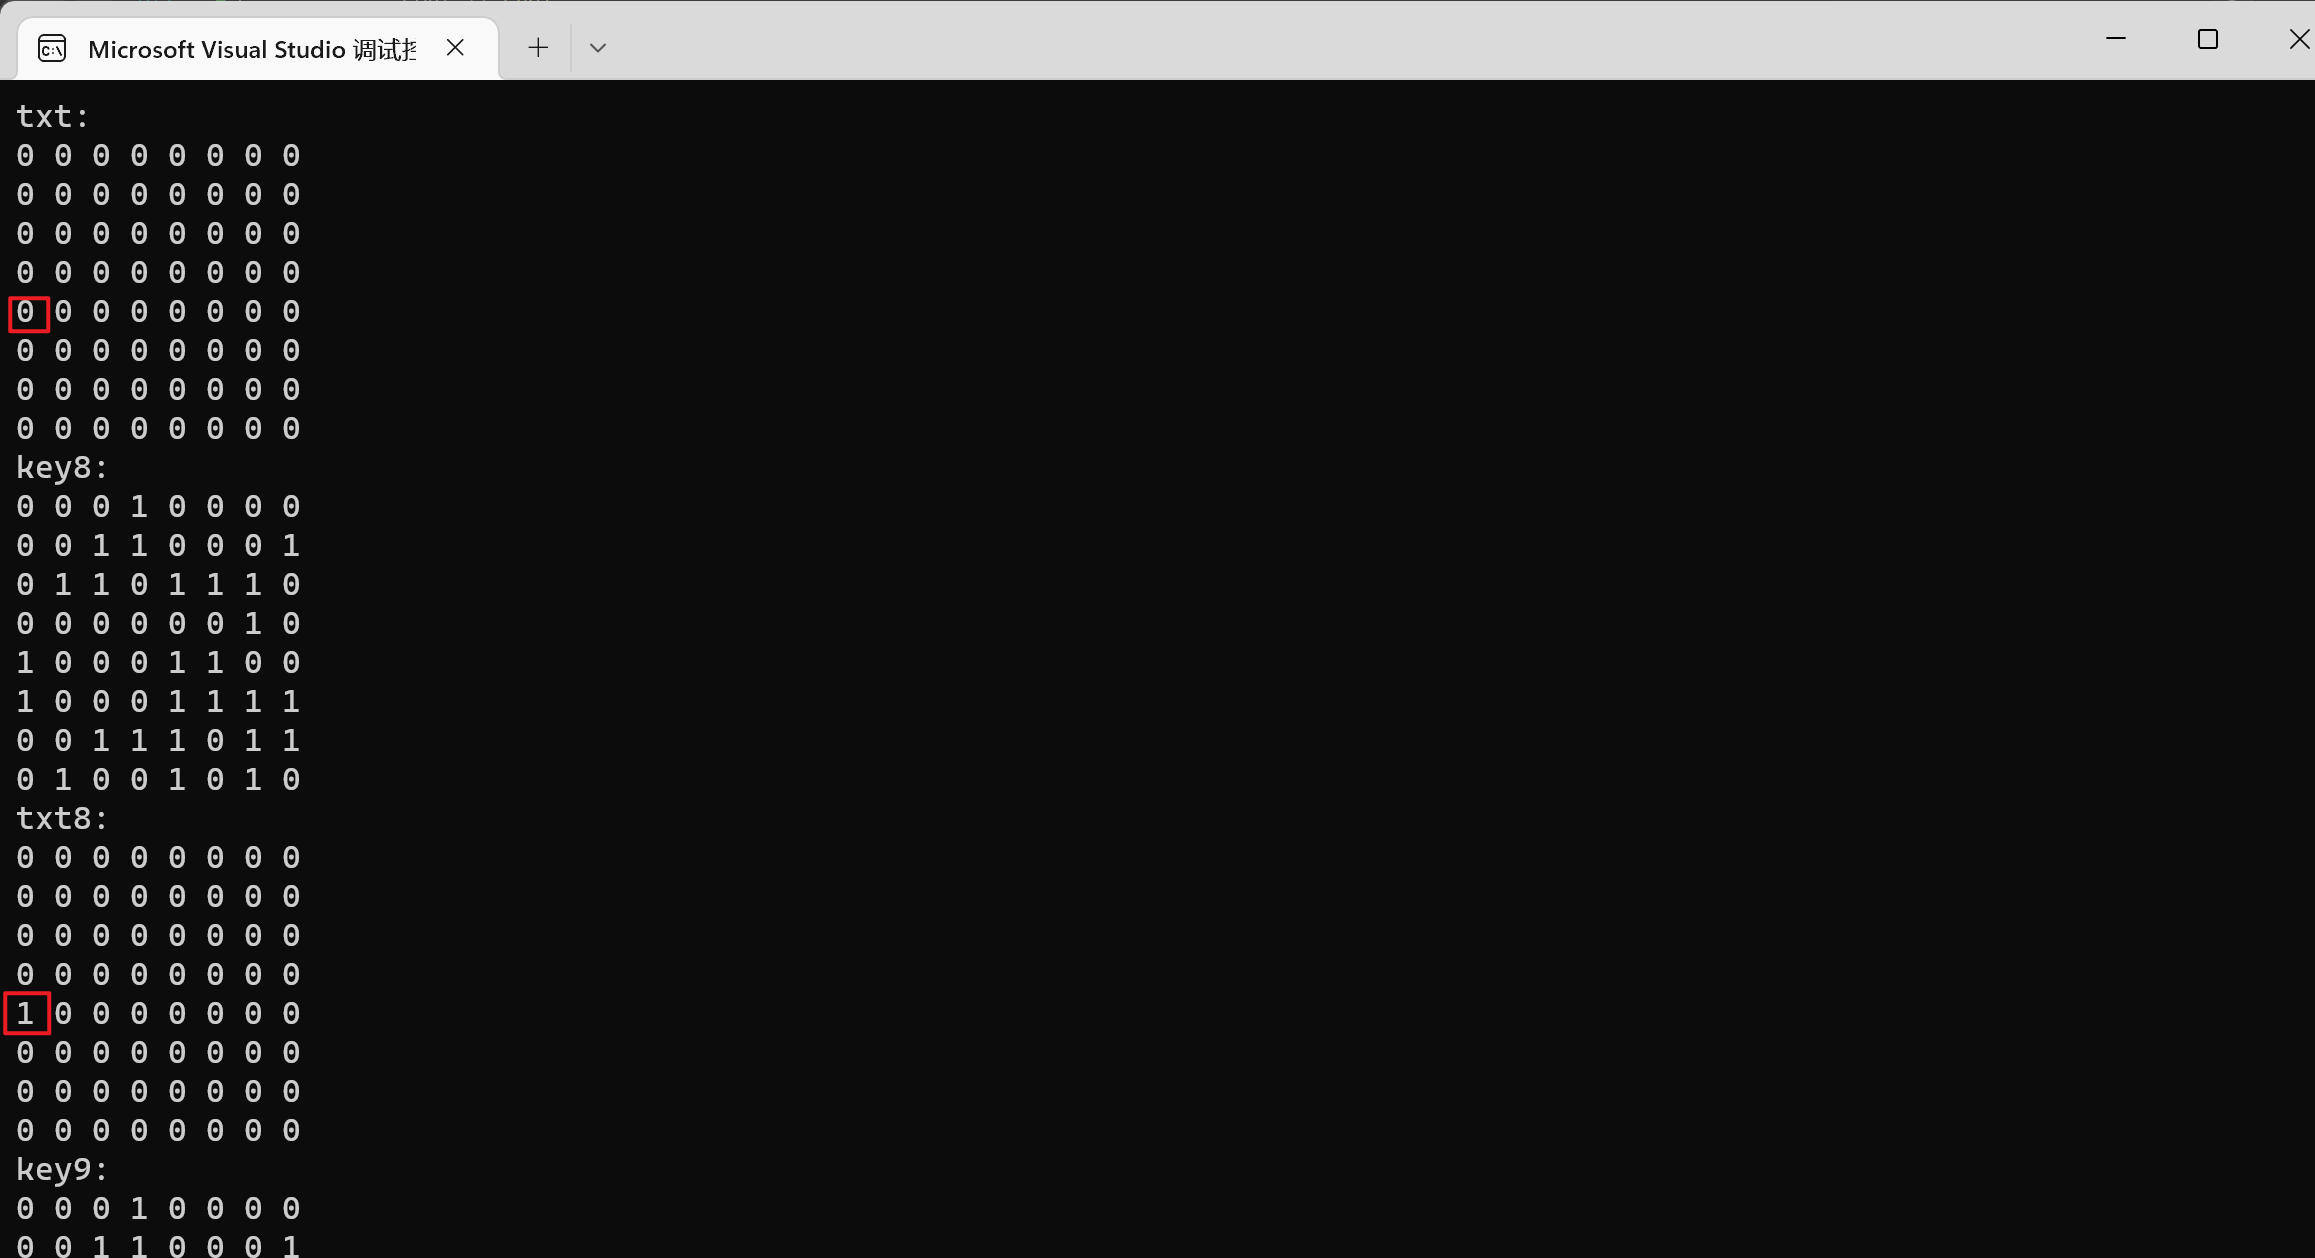
\includegraphics[height=10 CM]{figure/006}
	\caption{计算雪崩效应,改变txt的一位,key不变}
	\label{fig:计算雪崩效应,改变txt的一位,key不变}
\end{figure}
\begin{lstlisting}[language=c++]
// DES_CRYPTO.cpp : 
#include <iostream>
#include"des_test_data.h"
using namespace std;

int* child_key[16];//储存子密钥
//为了代码精简删掉表项,详情请见DES_CRYPTO.sln
const int IP_table[64] = {  };

const int IP_1_table[64] = { 
};
const int LS_table[16] = {
};
const int PC_1_table[56] = {};
const int PC_2_table[48] = { };
const int E_table[48] = { };
const int S_Box_table[32][16] = {  };
const int P_table[32] =
{
};

int* int2dec(int a)//a是int型,比如140
{
	int* b = new int[2];
	if (!a)
	b[0] = b[1] = 0;
	else
	{
		b[1] = a % 16;
		b[0] = a / 16;
	}
	return b;
}

void DEC2BIN(int a, int* b, int k)
{//将10进制数转换成2进制数,并用长度为4的int数组保存
	for (int i = 0; i < 8; i++)
	b[k + i] = 0;
	int* c = new int[2];
	c = int2dec(a);
	int temp;
	for (int i = 0; i < 2; i++)
	{
		if (!i)
		temp = k + 3;
		else
		temp = k + 7;
		while (c[i])
		{
			int j = c[i] % 2;
			c[i] /= 2;
			b[temp--] = j;
		}
	}
}

int* IP_replace(int* text)//IP置换
{
	int* temp = new int[64];
	for (int i = 0; i < 64; i++)
	{
		temp[i] = text[IP_table[i] - 1];
	}
	return temp;
}

int* IP_1_replace(int* text)//IP逆置换
{
	int* temp = new int[64];
	for (int i = 0; i < 64; i++)
	{
		temp[i] = text[IP_1_table[i] - 1];
	}
	return temp;
}

int* PC_1_replace(int* text)//压缩置换PC-1
{
	int k = 0;
	int* temp = new int[56];
	for (int i = 0; i < 56; i++)
	{
		temp[i] = text[PC_1_table[i] - 1];
	}
	return temp;
}

int* PC_2_replace(int* text)//压缩置换PC-2
{
	int* temp = new int[48];
	for (int i = 0; i < 48; i++)
	{
		temp[i] = text[PC_2_table[i] - 1];
	}
	return temp;
}

void LS(int* text,int K_num)
{//循环左移,K_num是第几个子密钥
	for (int j = 0; j < LS_table[K_num]; j++)
	{
		int* L = &text[0];
		int* R = &text[28];
		int temp1_1, temp1_2;
		temp1_1 = L[0], temp1_2 = R[0];
		for (int i = 0; i < 27; i++)
		{
			L[i] = L[i + 1];
			R[i] = R[i + 1];
		}
		L[27] = temp1_1;
		R[27] = temp1_2;
	}
}

int* f(int* R, int* K)
{
	int* temp = new int[48];
	for (int i = 0; i < 48; i++)
	{
		temp[i] = R[E_table[i] - 1];//E拓展
		if (temp[i] == K[i])//E拓展后与子密钥异或
		temp[i] = 0;
		else
		temp[i] = 1;
	}
	int* tmp = new int[32];
	for (int i = 0; i < 32; i++)
	tmp[i] = 0;
	for (int s = 0; s < 8; s++)//s代表盒号
	{
		int k = s * 6;
		//i,j用来定位在盒里的坐标s[i][j]
		int i= temp[k] * 2 + temp[k + 5];
		int j = temp[k + 1] * 8 + temp[k + 2] * 4
		 + temp[k + 3] * 2 + temp[k + 4];
		int num = S_Box_table[s * 4 + i][j];
		int N = s * 4 + 3;
		while (num)
		{
			int i = num % 2;
			num /= 2;
			tmp[N--] = i;
		}
	}
	int* tmpp = new int[32];
	for (int i = 0; i < 32; i++)
	{
		tmpp[i] = tmp[P_table[i] - 1];
	}
	return tmpp;
}

int main()
{
	//保存第0组数据,用于后续雪崩检验
	int key0[64], txt0[64], out0[64];
	cout << "num" << "\tmode" << endl;
	//20组数据,前10组为加密,后10组为解密
	for (int i = 0; i < 20; i++)
	{
		int k = 0;
		int* key = new int[64];//储存密钥
		int* txt = new int[64];//储存txt
		int* output = new int[64];//DES计算的结果
		int* out = new int[64];//正确的结果
		
		
//将key,txt,out转换成2进制,共64位,存储在长位64的int型数组里面
		for (int j = 0; j < 8; j++)
		{
			DEC2BIN((int)cases[i].key[j], key, k);
			DEC2BIN((int)cases[i].txt[j], txt, k);
			DEC2BIN((int)cases[i].out[j], out, k);
			k += 8;
		}
		//保存第0组的数据,用于后续雪崩效应的计算
		if (i == 0)
		{
			for (int i = 0; i < 64; i++)
			{
				key0[i] = key[i];
				txt0[i] = txt[i];
			}
		}
		int* temp = PC_1_replace(key);//压缩置换1
		for (int i = 0; i < 16; i++)
		{
			//循环左移
			LS(temp, i);
			//压缩置换2
			child_key[i] = PC_2_replace(temp);
		}
		txt = IP_replace(txt);//IP置换
		int* L = &txt[0];
		int* R = &txt[32];
		int j;//j用来区分加密和解密使用的子密钥不同
		if (cases[i].mode)
		{
			j = 0;
		}
		else
			j = 15;
		for (int k = 0; k < 16; k++)//16轮
		{
			int* tmpp;
			if (cases[i].mode)
			{//加密,子密钥正序使用0-15
				tmpp = f(R, child_key[j++]);
			}
			else//解密,子密钥逆序使用15-0
				tmpp = f(R, child_key[j--]);
			for (int i = 0; i < 32; i++)
			{//Ri=Li-1+f(Ri-1,Ki)
				if (tmpp[i] == L[i])
					L[i] = 0;
				else
					L[i] = 1;
			}
			int* temp = L;
			L = R;
			R = temp;
		}
		for (int i = 0; i < 32; i++)//左右交换
		{
			swap(L[i], R[i]);
		}
		output = IP_1_replace(txt);//IP逆置换
		if (i == 0)
		{
			for (int i = 0; i < 64; i++)
			{
				out0[i] = output[i];
			}
		}
	//用来判断计算得到的output与标准答案out是否一致
		bool t = true;
		for (int k = 0; k < 64; k++)
		{
			if (out[k] != output[k])
			{
				t = false;//不一致
				break;
			}
		}
		if (t)
			cout << cases[i].num << " \t" <<
			 cases[i].mode << "  \t成功" << endl;
		else
			cout << cases[i].num << " \t" << 
			cases[i].mode << "  \t失败" << endl;
	}
	
	//测试雪崩效应,选取第一组数据
	int num = 0;
//计算16次,前8次计算改变1bit密钥,不改变明文
//后8次计算改变1bit明文,不改变密钥
	for (int i = 0; i < 16; i++)
	{
		if (i % 8 == 0)
		num = 0;
		int* testkey = new int[64];
		int* testtxt = new int[64];
		int* testout = new int[64];
		if (i < 8)
		{
			for (int j = 0; j < 64; j++)
			{
				if (j == i * 8)
				{
					testkey[j] = (key0[j] + 1) % 2;
				}
				else
				{
					testkey[j] = key0[j];
				}
				testtxt[j] = txt0[j];
			}
		}
		else
		{
			for (int j = 0; j < 64; j++)
			{
				if (j == i * 4)
				{
					testtxt[j] = (txt0[j] + 1) % 2;
				}
				else
				{
					testtxt[j] = txt0[j];
				}
				testkey[j] = key0[j];
			}
		}
		int* temp = PC_1_replace(testkey);
		for (int i = 0; i < 16; i++)
		{
			LS(temp, i);
			child_key[i] = PC_2_replace(temp);
		}
		testtxt = IP_replace(testtxt);
		int* L = &testtxt[0];
		int* R = &testtxt[32];
		for (int k = 0; k < 16; k++)
		{
			int* tmpp;
			tmpp = f(R, child_key[k++]);
			for (int i = 0; i < 32; i++)
			{
				if (tmpp[i] == L[i])//Ri=Li-1+f(Ri-1,Ki)
				L[i] = 0;
				else
				L[i] = 1;
			}
			int* temp = L;
			L = R;
			R = temp;
		}
		for (int i = 0; i < 32; i++)//左右交换
		{
			swap(L[i], R[i]);
		}
		testout = IP_1_replace(testtxt);
		for (int i = 0; i < 64; i++)
		{
			if (out0[i] != testout[i])
			num++;
		}
		if (i == 7)
			cout << "The average of out changed 
			for changed 1bit of key is " <<
			 float(num / 8) << endl;
		if (i == 15)
			cout << "The average of out changed 
			for changed 1bit of txt is " <<
			 float(num / 8) << endl;
	}
}

\end{lstlisting}
%\begin{enumerate}
%	\item \textbf {预处理器:}处理源代码中以\#开始的预编译指令,例如展开所有宏定义、插入\#include指向的文件等,以获得经过预处理的源程序。
%	
%	\item \textbf {编译器:}将预处理器处理过的源程序文件翻译成为标准的汇编语言以供计算机阅读。
%	
%	\item \textbf {汇编器:}将汇编语言指令翻译成机器语言指令,并将汇编语言程序打包成可重定位目标程序。
%	
%	\item \textbf {链接器:}将可重定位的机器代码和相应的一些目标文件以及库文件连接在一起,形成真正能在机器上运行的目标机器代码。
%\end{enumerate}

%\begin{figure}[thbp!]
%	\centering
%	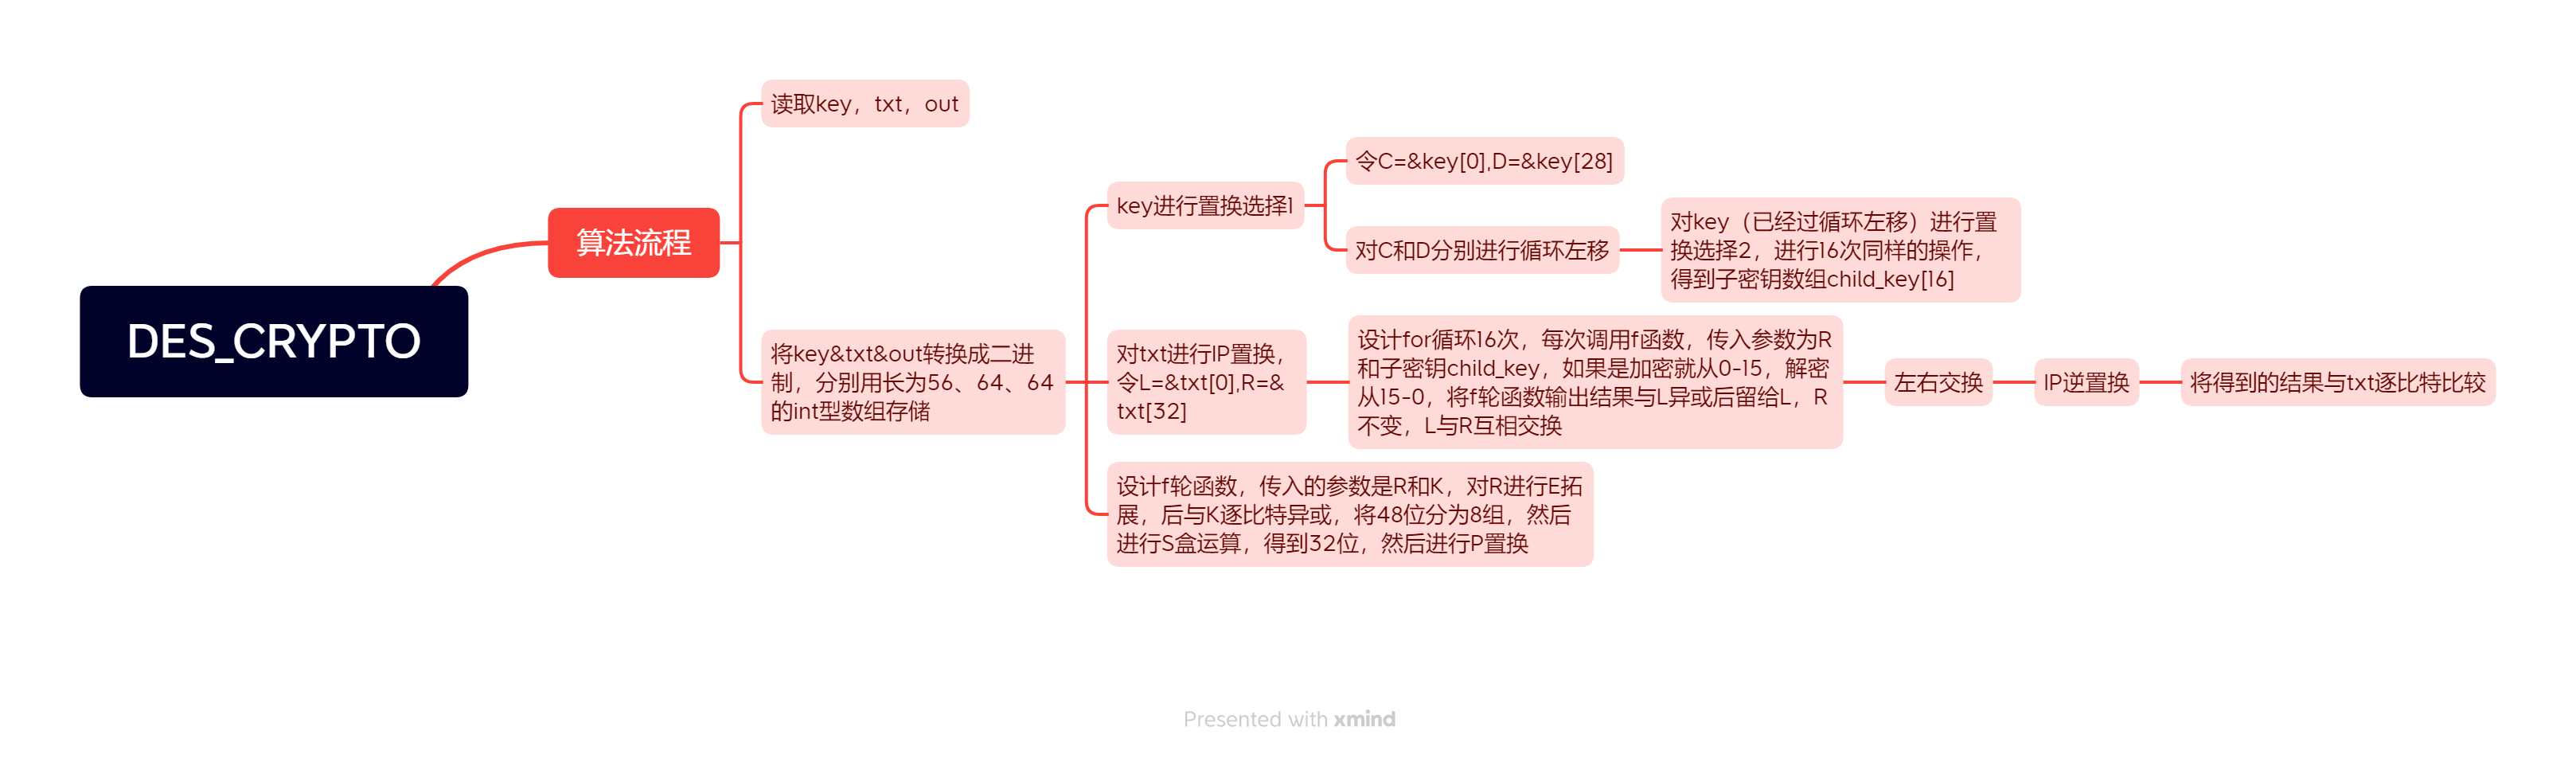
\includegraphics[height=6.8 CM]{figure/001}
%	\caption{语言处理过程图示}
%	\label{fig:语言处理过程图示}
%\end{figure}

























